
\section{Solr}

\subsection{Installation}

Als Systemvoraussetzungen ist eine Java Version $> 8$ gegeben. Ich habe mich hierbei für OpenJDK 11 entschieden. 
Nach dem ersten Starten wurden 2 Warnungen gemeldet, dass die User-Limits für Solr zu gering sind \ref{lst:warningSolr}. Nachdem diese entsprechend erhöht wurden, verschwanden die Warnungen.

\begin{lstlisting}[language=bash, frame=single, label={lst:warningSolr}] 
  *** [WARN] *** Your open file limit is currently 1024.
  It should be set to 65000 to avoid operational disruption.

  *** [WARN] ***  Your Max Processes Limit is currently 63918.
  It should be set to 65000 to avoid operational disruption.
\end{lstlisting}

Um Solr im Entwicklermodus auszuführen, kann das entpackte Programm einfach mit \path{bin/solr start} gestartet werden. 
Bei der richtigen Installation installiert sich Solr als Service und legt einen eignen Nutzer an. Ein entsprechendes Installations-Skript findet sich dafür im entpackten Solr-Ordner.

\subsection{Indexierung}

Um mit der Indexierung starten zu können, muss zuerst in sogenannter Core erstellt werden. Dieser ist ein Index mit dazugehörigen Transaktions-Log und den Konfigurationsdateien. Nur mit diesen ist es möglich Dateien zu indexieren und auf ihnen zu suchen. Nach der Erstellung lässt sich der Core nun auch über die Oberfläche einsehen und zum Teil konfigurieren.

Damit Solr nun die Daten von der Datenbank liest, muss ein DataImportHandler (DIH) \ref{lst:dih} geschrieben werden. In diesen werden die Daten, welche Indexiert werden sollen, mit MySQL-Queries eingelesen. Das System setzt dabei auf eine XML-Struktur mit sogenannten Entitys. Diese besitzen jeweils mehre Attribute, wie den Namen, welcher auf der Oberfläche zur Indexierung angezeigt wird, den MySQL-Query mit dem die Daten gelesen werden und einen Delta-Query, welcher dazu dient, nur die neuen Einträge zu laden. Der Delta-Query benötigt hierbei eine eigene Zeitstempel-Spalte in der Datenbank, welche angezeigt, wann die Spalte das letzte Mal editiert wurde. Da die Tabellen im Projekt eine solche Spalte nicht besitzen können die Delta-Querys nicht getestet werden. 
Innerhalb des Entity Elements gibt es entweder weitere Entitys, dazu gleich mehr, oder Field-Elemente. Diese besitzen ein Attribut, welches die Spalte der Tabelle ausweist und einen Namen, der das zugehörige Solr-Schema-Element ausweist. 
Entitys können unbegrenzt ineinander verschachtelt werden. Damit Änderungen an einer verschachtelten Entity nach oben richtig weitergegeben werden, gibt es Parent-Delta-Querys. Diese geben die betroffenen Werte an die übergeordnete Entity weiter. Dafür führt der Parent-Delta-Query einen Aufruf an die überliegende Entity-Tabelle aus, in der er mithilfe der Fremdschlüssel-IDs in den betroffen Zeilen herausfindet.

Der DataImportHandler muss, bevor er benutzt werden kann, jedoch noch mit dem Core verbunden werden, dafür wird er, zusammen mit einem JDBC-Treiber in die solrconfig.xml eingetragen. Bei den JDBC-Treiber habe ich mich bei diesem Beispiel für den Treiber von MariaDB entschieden. Damit es nicht deswegen zu Laufzeit-Unterschieden bei der Indexierung kommen kann, werde ich diesen Treiber bei allen Systeme, dies es zulassen, den MariaDB-Treiber verwenden.

\begin{lstlisting}[language=xml, frame=single, label={lst:dih}, 
    morekeywords={entity,query,deltaQuery,parentDeltaQuery,field,column, name}] 
    <entity name="lemma" 
      query="select * from lemma" 
      deltaQuery="select eid from lemma 
        where last_modified > '${dataimporter.last_index_time}'"> 
		<field column="bezeichnung" name="bezeichnung" />
    [...]
    <entity name="lemma_gnd" 
      query="select * from lemma_gnd where fk_lemma='${lemma.id}'"
      deltaQuery="select * from lemma_gnd 
        where last_modified > '${dataimporter.last_index_time}'"
      parentDeltaQuery="select * from lemma 
        where id=${lemma_gnd.fk_lemma}">
			
        <entity name="gnd" 
          query="select * from gnd where id = '${lemma_gnd.fk_gnd}'"
          deltaQuery="select * from gnd 
            where last_modified > '${dataimporter.last_index_time}'"
          parentDeltaQuery="select * from lemma_gnd where fk_gnd=${gnd.id}">
          <field column="nummer" name="gnd_nummer" />
          <field column="schlagwort" name="gnd_schlagword" />
          [...]
        </entity>
      </entity>  
    </entity>
\end{lstlisting}

Wie schon eben angesprochen, muss das Solr-Schema für die entsprechende Elemente auch angepasst werden. Dieses Schema dient dazu die Dateitypen für eine möglichst gute Indexierung auszuweisen. Dafür wird zuerst der Dateityp für die Tabellen-Spalte angegeben. Hierbei werden bei den Grundtypen, zum Beispiel unter anderem String und Text\_de gelistet. Ohne genauer darüber nachzudenken, habe ich angenommen, dass beide gleichwertig sind und nur für spätere Abfragen auf Sprachen eine Relevanz besitzen. Als ich allerdings eine Abfrage stellte, die alle Lemmata mit den Buchstaben S finden sollte, bekam ich mehr Ergebnisse als erwartet. Dies liegt daran, dass Text\_de, das Feld aus Volltext ausweist. 
Bei Volltexten wird jedes Wort einzeln betrachet und so kamen Lemma, in welchen irgendein Wort mit S begann in meine Auflistung. 

Auch muss darauf geachtet werden, ob der Typ String oder Strings angegeben wird. Letzteres weist das Feld als multiValued aus. Dieser bildet eine 1 zu N Beziehung ab. So kann man zusammen mit der Verschachtelung des DataImportHandlers auch N zu M Beziehungen abbilden.

Es gibt mehrere Möglichkeiten diese Einträge auszuweisen. In diesem Fall habe ich die Einträge über die Administrations-Oberfläche angelegt. Es ist allerdings auch möglich eine eigene Schema-Datei zu erstellen. Diese Methode soll allerdings nicht mehr verwendet werden, da es die Möglichkeit gibt, diese Einträge per API einlesen zu lassen. Dadurch wird direkt überprüft, ob die Einträge formal stimmen. So können keine fehlerhaften Schemata gebaut werden. Die Einträge, welcher über die API oder die Administrations-Oberfläche gestellt werden, werden in einer Datei namens managed\_schema \ref{lst:managedSchema} im XML-Format angelegt.


\begin{lstlisting}[language=xml, frame=single, label={lst:managedSchema}, 
    morekeywords={type,uninvertible,indexed,stored,field,multiValued, name}] 

    [...]
    <field name="ddc_webdewey_is_checked" type="boolean" 
        uninvertible="false" indexed="true" stored="true"/>
    <field name="description" type="text_de" uninvertible="false" 
        multiValued="true" indexed="true" stored="true"/>
    <field name="erweiterung" type="text_de" 
        uninvertible="false" indexed="true" stored="true"/>
    [...]

\end{lstlisting}

Die Indexierung lief eine Minute und 34 Sekunden für rund 14 Tausend Einträge \ref{img:solrIndexTime}. Dabei wurde der gegebene Arbeitsspeicher nicht komplett ausgenutzt, was darauf schließen lässt, dass die Datenbank der limitierende Faktor war. Die hohe Anzahl der Abfragen ist darauf zurückzuführen, dass Solr keine Joins verwendet, sondern bei jeder verschachtelten Entity die gesamten Tabellen wieder und wieder passenden Einträgen durchsucht.

\begin{figure}
	\centering
	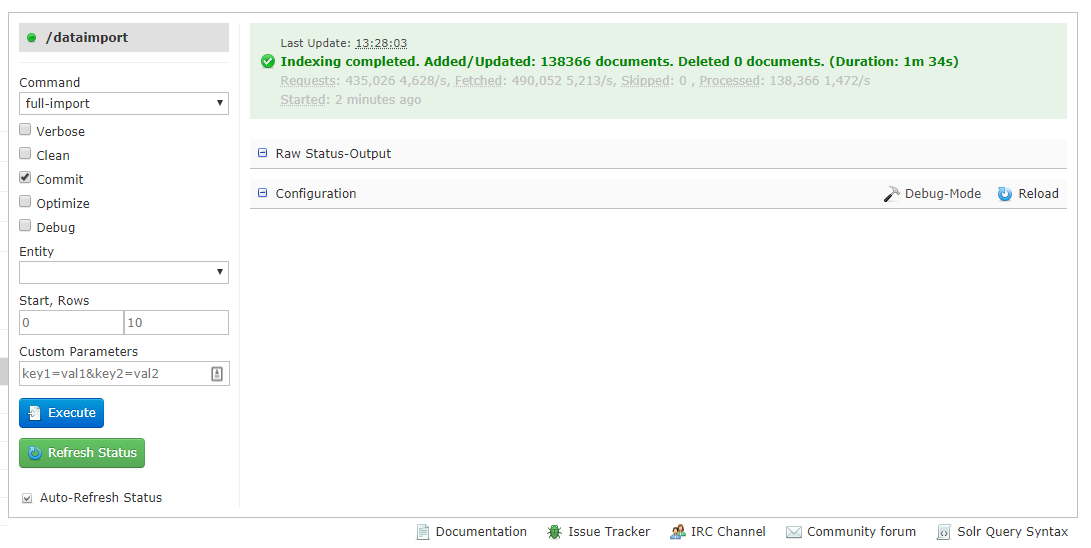
\includegraphics[width=1\linewidth]{images/solr_indexing_time.png}
	\caption{Oberfläche der Indexierung mit Laufzeit.}
	\label{img:solrIndexTime}
\end{figure}

\subsection{Oberfläche}

Der Startseite des Solr-Systems bietet direkten Einblick in auf die Auslastung des Systems \ref{img:solrInterface}. Der Fehler-Log ist auch sehr einfach mit einem Klick zu erreichen. Um an die Statistiken von dem aktuellen Core zu kommen, kann dieser aus einen Drop-Down-Menu ausgewählt werden. Positiv anzumerken ist, dass es möglich ist, Schema Einträge direkt in der Weboberfläche zu löschen und anzulegen. Leider ist es jedoch nicht möglich, den DataImportHandler direkt zu verändern, ohne weitere Einstellungen im System vorzunehmen. Es gibt eine Möglichkeit Querys direkt über den Web-Client zu senden, was zum Testen und debuggen sehr nützlich ist. Auch bei der Indexierung kann ein Debug-Modus dazu geschaltet werden \ref{img:solrIndexTime}. Zudem besteht die Möglichkeit die Konfigurationsdateien des Cores auf der Weboberfläche einzusehen. Die Dateien dort direkt zu editieren, ist jedoch nicht möglich.
Es gibt keine Möglichkeit Updates direkt über die Weboberfläche einzuspielen, zudem ist die Seite auch nicht responsive geschrieben. 

\begin{figure}
	\centering
	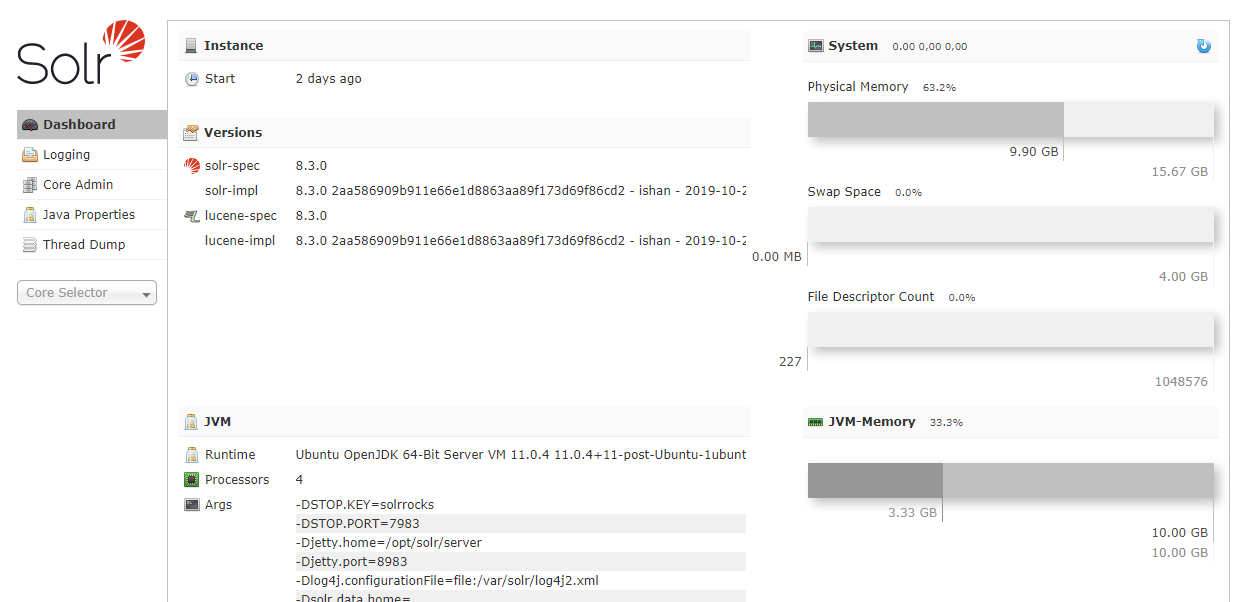
\includegraphics[width=1\linewidth]{images/solr_interface.png}
	\caption{Startseite der Weboberfläche von Solr.}
	\label{img:solrInterface}
\end{figure}


\subsection{Dokumentation}

Die Dokumentation war bei diesem kurzen Test meine Hauptquelle. Die Installation ist dort genau beschrieben. Positiv aufgefallen ist mir dabei vor allem die genaue Beschreibung der Systemanforderungen. Es wurde diverse Java-Versionen getestet und dort aufgeführt. 
Generell gibt es für alle Themen eine kleine Übersichtsseite, welche die grundlegenden Funktionen erklärt, ohne sich dabei in Details zu verlieren. 
Die Seite für den DataImportHandler hat anhand eines Beispiels gut die Struktur erklärt. Allerdings wäre ein Verweis, dass für die DataImportHandler-Attribute noch extra ein Solr-Schema-Attribut benötigt wird, schön gewesen. Dies habe ich erst durch einen Blog \cite{IqubalMustafaKaki.2016} herausgefunden und richtig verstanden. 
Die Dokumentation ist, soweit ich das gesehen habe, gut bebildert und bietet einen guten Einstiegspunkt in das System.

\subsection{Absetzen einer Anfrage und Integration in PHP}

Um nicht direkt mit der JSON-API arbeiten zu müssen, gibt es diverse Bibliotheken, die ein wenig der Arbeit abnehmen. Eine der größten ist hierbei Solarium, welches sich mit Composer installieren lässt. Dies passt sehr gut zum Dietrich-Online Projekt, da auch dieses auf Composer setzt. 
Die Query ist herbei sehr einfach, da die Daten beim Import schon dementsprechend indexiert wurden.

\begin{lstlisting}[language=php, frame=single, label={lst:SolrPhp}, 
  morekeywords={type,uninvertible,indexed,stored,field,multiValued, name}] 

  [...] # Imports and variable declarations

  $config = array(
      'endpoint' => array(
          'localhost' => array(
              'host' => '136.199.34.55',
              'port' => 8983,
              'core' => 'dietrich'
  )));
  $queryText = 'original_bezeichnung:S*';
  $solr = new Client($config);
  $query = $solr->createSelect();
  $query->setQuery($queryText);
  $query->setRows(2147483647); 
  [...] # Loop with Timer
  $resultSet = $solr->select($query);
  $count = $resultSet->count();
  [...] # Output Runtime
\end{lstlisting}

Interessant bei der Verbindung ist, dass die Anzahl der Zeilen die von Solr geladen werden, standardmäßig auf 10 limitiert sind. Erst mit setRows kann die Anzahl erhöht werden. Ich für diesen Test den maximalen Integer-Wert gewählt, um immer alle Ergebnisse zu bekommen. Damit ich nun einen guten Median-Wert erhalte habe ich die Abfrage 100 mal laufen lassen. Dabei lief die Abfrage durchschnittlich 1.01 Sekunden um die 15838 Ergebnisse herauszusuchen. Eine Vergleichstabelle, wie sich Solr dabei mit den anderen Suchmaschinen schlägt, finden Sie hier. !!VERGLEICH ANFÜGEN!!
